% Shared body for both the one-column (main.tex) and two-column (main_twocol.tex)
% builds. Figure width is controlled by \figw, defined per-wrapper (\linewidth in 2-col,
% a fraction of \linewidth in 1-col). Wide figures use \figstar (figure* in 2-col,
% figure in 1-col), also defined per-wrapper.

\section{Introduction}
Ask a spectator where the ball is in a match photo with the ball digitally erased and
they will often point close to the truth: the players' stances and motion give it away.
Can machines do the same, and what exactly is the signal? We formalize \emph{hidden-ball
localization}---predict the ball's image (or field) position from players only---as a
probe of spatial inference, and use it to contrast frontier VLMs against a tiny
task-specific model, then to reverse-engineer what makes the task solvable.

Our contributions:
\begin{itemize}
  \item A \textbf{de-biased benchmark} ($n=260$) on SoccerNet-Tracking broadcast frames
  with the ball removed by LaMa inpainting~\cite{suvorov2022lama} and a leak control (a VLM
  flags residual ball/artifact cues; $12.7\%$ of items, which we can exclude),
  balancing ball position to neutralize the ball-following camera. None of four current
  frontier VLMs (GPT-5.4, Claude Opus 4.8, Sonnet 4.6, Llama-4-Maverick) beats a
  camera-center baseline on off-center balls.
  \item A \textbf{scale-up to 12 matches across two leagues} showing interpretable
  geometry recovers the deep specialist, and that the localization signal is
  \emph{collective motion}, with the \emph{still ball} as the model's blind spot.
  \item A \textbf{cross-sport analysis} placing the zero-shot transfer asymmetry in the
  velocity channel, and a \textbf{calibration study} exposing over-confidence on exactly
  the hard, off-center cases.
\end{itemize}

\section{Related Work}
\textbf{Ball from players.} Recovering the ball from player configuration is an established
task: Maksai et al.~\cite{maksai2016players} denoise ball trajectories under physical and
interaction constraints; BallRadar~\cite{kim2023ballradar} regresses the full ball trajectory
from tracking with a permutation-invariant set model plus a possession stage;
TranSPORTmer~\cite{capellera2024transportmer} folds ball inference into a holistic multi-agent
transformer. Our contribution is not \emph{whether} this is possible but a strictly
counterfactual, camera-de-biased benchmark, a minimal-signal geometric dissection, a
velocity-scale transfer analysis, and a calibration blind spot---not a point trajectory.
\textbf{Interpretable spatial value.} The velocity-weighted centroid is a lightweight cousin
of pitch control: Spearman's pass- and space-value models~\cite{spearman2017physics,spearman2018beyond}
and the space-occupation line of Fern\'andez \& Bornn~\cite{fernandez2018wide} are the field's
standard interpretable models of who controls space toward the ball.
\textbf{VLM spatial reasoning.} Frontier VLMs~\cite{achiam2023gpt4} are documented to fail
fine spatial relations (What'sUp~\cite{kamath2023whatsup}, BLINK~\cite{fu2024blink}) and, in
sports, both understanding (SPORTU~\cite{xia2025sportu}) and visual grounding---SoccerLens
~\cite{elsharkawi2026soccerlens} finds soccer VLMs stay below $50\%$ grounding, drifting to
spurious regions. Those benchmarks ask whether a model attends to the right pixels; we
instead \emph{remove} the object and de-bias the camera, so the task measures spatial
\emph{inference} from configuration rather than perception or dataset priors. \textbf{Method building blocks.} Player/ball tracks from
SoccerNet-Tracking~\cite{cioppa2022soccernet}, Metrica~\cite{metrica2020},
SkillCorner~\cite{skillcorner2020}, NBA SportVU~\cite{sportvu2016} (ball as target only); a
permutation-invariant Deep Set~\cite{zaheer2017deepsets}; a mixture-density
head~\cite{bishop1994mdn}; persistent homology~\cite{ripser2018} features (which add nothing
over plain geometry).

\section{Task, Data, and Method}
\textbf{Task.} Given players (image or field coordinates, with velocities) at one instant,
predict the ball position; the ball is never observed at input. Error is the median
Euclidean distance in normalized coordinates.
\textbf{Image space.} From SoccerNet-Tracking we sample frames, remove the ball with a
speed-padded mask + LaMa, and verify non-leakage with a VLM leak check. We balance items
by distance of the ball from frame center (near/mid/far) to defeat the camera-center
baseline. The scaled set is 260 items (80 near / 60 mid / 120 far), drawn from the
SoccerNet-Tracking test and train splits with a per-clip cap.
\textbf{Field space.} Metrica + SkillCorner (soccer, two leagues) and NBA SportVU
(basketball) give ground-truth player and ball tracks; per-player features are
$(x,y,v_x,v_y,\text{team})$ over a 1\,s window.
\textbf{Models.} (i) frontier VLMs (GPT, Claude family) prompted to output ball
coordinates on the inpainted image; (ii) a Deep Sets specialist ($\sim$13k params, $\sim$50\,kB); (iii)
an interpretable model: eleven named geometric features + gradient-boosted trees; (iv)
a mixture-density head for uncertainty. Baselines: frame center (B0) and the (velocity-
weighted) player centroid (B1).

\section{Results}
Table~\ref{tab:overview} summarizes the six findings; each is detailed below.

\begin{table}[h]\centering\small
\begin{tabular}{@{}p{0.30\linewidth}p{0.62\linewidth}@{}}
\toprule
Finding & Key result (12 matches / $n{=}260$) \\
\midrule
VLMs vs.\ specialist (far) & specialist wins $68\%$ vs.\ camera; no VLM clears chance (GPT-5.4 $52$, Opus $44$, Sonnet $36$, Llama-4 $34$) \\
Geometry $\approx$ deep & geo $0.099$ recovers $91\%$ of tuned deep $0.087$; $>$ pitch control $0.186$, centroid $0.213$ \\
Signal is motion & removing velocity costs $0.035$, 12/12 \\
Stillness blind spot & still ball hardest; velocity useless when still (12/12); in-flight direction $32^\circ$ \\
Cross-sport transfer & deep asymmetric (s$\to$b $0.32$, b$\to$s $0.21$), geo symmetric; asymmetry in the velocity channel \\
Calibration & globally calibrated ($r{=}{+}0.20$) but over-confident on loose balls \\
Topology & adds nothing over geometry ($0.258$ vs.\ $0.111$) \\
\bottomrule
\end{tabular}
\caption{Overview of results.}
\label{tab:overview}
\end{table}

\subsection{Frontier VLMs do not solve the off-center cases}
On the de-biased set ($n=260$: 80 near / 60 mid / 120 far), we prompt current frontier
VLMs to output ball coordinates on the LaMa-inpainted image. The decisive bin is
\emph{far}: off-center balls where the camera-center baseline (error $0.362$) is weak.
None of the four current frontier VLMs reliably beats that baseline there. By win-rate (the
fraction of items whose prediction is closer to the ball than the frame centre) none clears
it: GPT-5.4 $52\%$ (CI $[43,62]$) and Claude Opus 4.8 $44\%$ ($[35,53]$) are indistinguishable
from chance, while Claude Sonnet 4.6 $36\%$ ($[28,45]$) and Llama-4-Maverick $34\%$ ($[25,42]$;
Fig.~\ref{fig:vlm}) are significantly below it. Even GPT-5.4, the strongest, only ties the
baseline on median error ($0.354$ vs.\ $0.362$), and far-bin correlation with the truth is
weak ($r_y\le0.29$). VLMs post good medians only on near-center items, where the camera has
already done the work. The result is not an inpainting artifact: the leak control flags
$12.7\%$ of items with residual ball/artifact cues, and excluding them leaves the far-bin
win-rates essentially unchanged (GPT $54\%$, Opus $42\%$, Sonnet $34\%$, Llama $32\%$). As a head-to-head on the
\emph{same} far items and the same input (player positions), a small specialist trained by
5-fold cross-validation wins $68\%$ (CI $[59,76]$, median $0.289$)---clearing the baseline
the VLMs cannot (Fig.~\ref{fig:vlm}); an image-space player centroid manages only $16\%$,
so the specialist is not merely following the crowd.

\begin{figure}[t]\centering
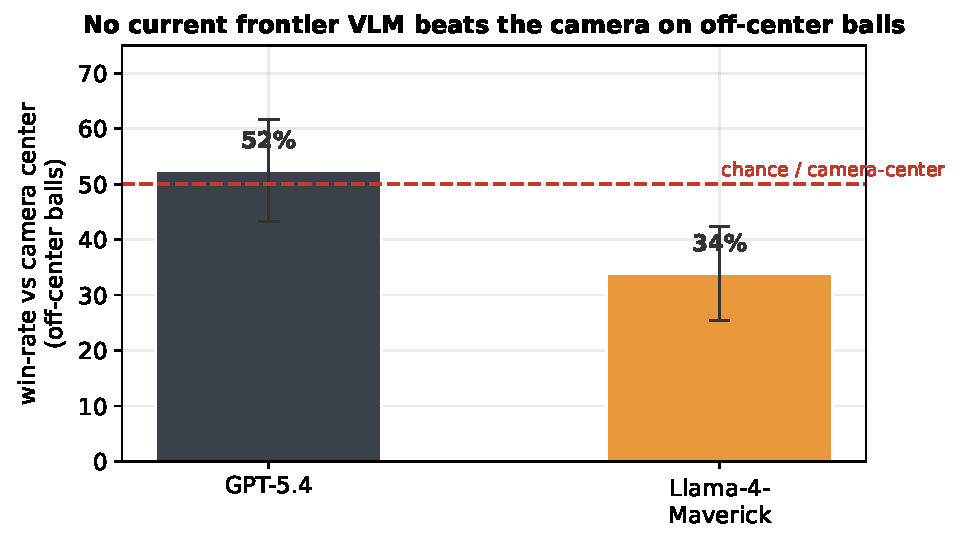
\includegraphics[width=\figw]{figures/fig1_vlm.pdf}
\caption{Off-center (far) balls, same $n=120$ items (Llama-4 $n=118$), 95\% bootstrap CIs.
A positions-only specialist trained on these items (5-fold CV) beats the camera-center
baseline (dashed); none of the four current frontier VLMs does. GPT-5.4, Opus 4.8, and
Sonnet 4.6 were run single-shot via the Claude/OpenAI interfaces available to us (Claude
via the agent harness; see Limitations), Llama-4 via Azure.}
\label{fig:vlm}
\end{figure}

\subsection{The specialist computes interpretable geometry}
Leave-one-match-out over 12 soccer matches (Metrica + 10 SkillCorner, 250k frames),
eleven interpretable geometric features fed to a gradient-boosted tree recover
$\mathbf{91\%\pm3\%}$ of a tuned, multi-seed Deep Sets specialist's gain over the centroid
baseline (Fig.~\ref{fig:core}). A single feature---the velocity-weighted centroid---
carries the localization; the remaining features add only marginal gains, and a tidy
motion-ray convergence point barely helps. Crucially, this is not beating a strawman: the
learned geometry also far outperforms pitch control~\cite{spearman2018beyond}, the field's
standard physical control model, which we run as a baseline ($0.186\pm0.010$; itself better
than the naive centroid, 12/12). The deep model retains a small edge over the learned
geometry ($0.087$ vs.\ $0.099$, 12/12 matches), so the reading is that most---not all---of
what the black box learns is a legible geometric quantity, not that geometry replaces deep
learning.

\begin{figure}[t]\centering
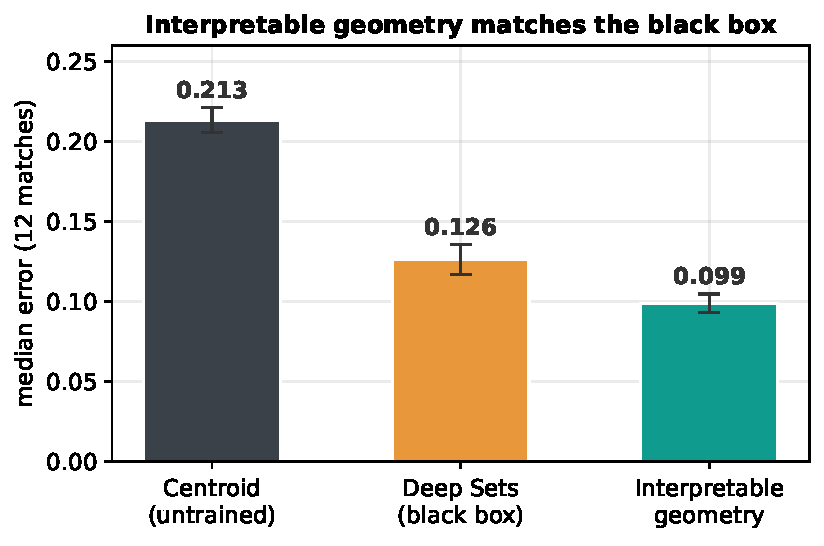
\includegraphics[width=\figw]{figures/fig2_core.pdf}
\caption{Leave-one-match-out across 12 matches, two leagues (mean$\pm$std). Ascending skill:
naive centroid ($0.213$), pitch control ($0.186$, the standard physical model), eleven
interpretable geometric features ($0.099$), tuned multi-seed Deep Sets ($0.087$;
across-seed std $0.002$). The learned geometry recovers $91\%$ of the deep model's gain over
the centroid and far outperforms pitch control---most of what the specialist learns is a
legible geometric quantity, chiefly the velocity-weighted centroid.}
\label{fig:core}
\end{figure}

\subsection{The signal is collective motion; stillness is the blind spot}
Removing the velocity channel costs $0.035\pm0.002$ in median error and hurts in
\textbf{12/12} matches (Fig.~\ref{fig:mech}). Splitting by ball speed, error is highest for the
\emph{still} ball ($<2$\,m/s), and velocity's contribution collapses there
($+0.016$ vs.\ $+0.041$ moving; less-when-still in 12/12). The worst still balls sit
centrally, far from the player mass (coupling---the ball's distance to the velocity-weighted
player centroid---correlates with error, $+0.53$ to $+0.65$): a still ball no one is near or
moving toward is undetermined. In flight, the ball's
\emph{direction} of travel is readable from players well above chance (leave-one-match-out
over the 12 matches: $32^\circ$ median angular error vs.\ $90^\circ$ chance; $61\%$ of fast
balls pinned within a $45^\circ$ cone, 12/12). A label-shuffle control confirms the geometry
model's skill is genuine inference, not marginal-distribution structure: training on
frame--ball pairs with the ball drawn from a random other frame yields $0.403$ error, far
worse than the real $0.099$ (and than the centroid's $0.213$), in 12/12 matches.

\begin{figure}[t]\centering
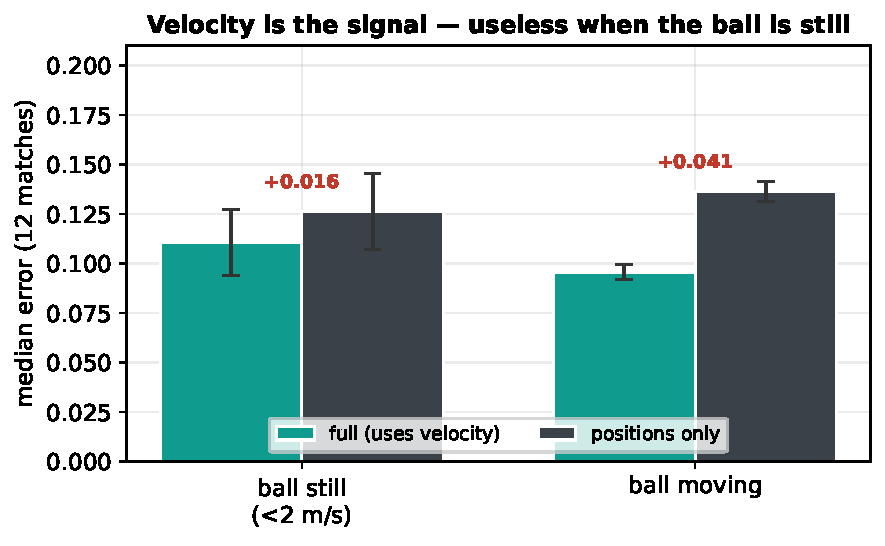
\includegraphics[width=\figw]{figures/fig3_mechanism.pdf}
\caption{Velocity ablation, still vs.\ moving ball, 12 matches (mean$\pm$std). Removing
velocity (teal$\to$graphite) costs $+0.041$ when the ball moves but only $+0.016$ when
it is still: with no motion there is no velocity signal to read. Velocity's contribution
is smaller when still in 12/12 matches.}
\label{fig:mech}
\end{figure}

\subsection{Cross-sport transfer and the velocity-scale mechanism}
Trained on one sport and tested zero-shot on the other under the same
leave-one-match-out protocol as in-domain (12 soccer matches, 250k frames; 6 basketball
games, 231k frames; tuned Deep Sets, 3 seeds), transfer is imperfect both ways. In
absolute error the Deep Sets transfers \emph{asymmetrically}---basketball$\rightarrow$soccer
$0.210$ vs.\ soccer$\rightarrow$basketball $0.319$---while the interpretable geometry model
transfers \emph{symmetrically} ($0.221$ vs.\ $0.217$), so the asymmetry is a property of the
distributed representation, not of the task.\footnote{A leakage-prone random split (adjacent
frames of a match in both train and test) had exaggerated the deep gap to $0.196$ vs.\ $0.395$;
the clean leave-one-match-out protocol narrows it.} The Deep Sets' asymmetry lives in the
velocity channel: removing velocity roughly halves the directional gap (absolute
$0.109\rightarrow0.056$), and flattens the asymmetry for both models on a penalty-ratio metric
(zero-shot error over in-domain error, differenced across directions, so $0$ is symmetric):
deep $-0.23\rightarrow-0.07$, geometry $-0.75\rightarrow-0.08$. A basketball court is $\sim$1/16
the area of a pitch ($\sim$4$\times$ shorter linearly), so in normalized coordinates
velocities differ 3--4$\times$; the learned use of velocity is scale-bound and does not
cross, while scale-free positions do.

\subsection{Calibration and the blind spot}
A mixture-density head is globally calibrated (declared uncertainty tracks error,
$r=+0.20$, monotonic) but over-confident on loose balls: as the ball moves away from the
player mass its actual error rises (corr $+0.20$, CI $[0.18,0.22]$) while its declared
uncertainty \emph{falls} (corr $-0.17$, CI $[-0.19,-0.15]$)---opposite-signed,
non-overlapping. It is most confident exactly where it errs most, and these are the same
off-center balls the VLMs fail.

\subsection{Topology adds nothing}
Persistent homology features (loop centres, largest empty Delaunay circles, persistence
statistics) do not beat plain geometry (topology-only 0.258 vs.\ geometry 0.111 in soccer)
and are ignored when concatenated to it---a negative result fixed by a threshold set in
advance (topology must beat the geometry model).

\section{Discussion and Limitations}
The capability frontier VLMs lack here is narrow and identifiable---reading collective
motion---and it is cheap: a 50\,kB set function learns it, and it reduces to a
velocity-weighted centroid. Limitations: the field-space specialist and image-space
specialist use ground-truth player positions (an information ceiling), and the specialist
vs.\ VLM head-to-head (Fig.~\ref{fig:vlm}) shares items and input but the specialist is
still handed clean positions; the VLM benchmark is a focused $n$ with bootstrap CIs, and
the frontier VLMs are versioned snapshots whose behaviour drifts, so ``no current VLM beats
the baseline'' is a dated claim, not a general one. The four VLMs were also run through
different interfaces---GPT-5.4 and Llama-4-Maverick via Azure APIs, Claude Opus 4.8 and
Sonnet 4.6 single-shot through the Claude Code agent harness (Azure had no Claude quota and
our Anthropic API credit was exhausted); the harness constrains each call to one image and
the same prompt, but is not identical to a raw API call, a caveat for the two Claude rows.
In the far bin, ``off-center ball'' is partly entangled with unusual (transition/wide)
camera framing. Learned models are single-architecture; the reported $\pm$ is inter-match,
with inter-seed variance separately small ($\le0.002$).

\paragraph{Data and reproducibility.} Code, feature definitions, and the pinned inpainting
pipeline are released. Player/ball tracks come from SoccerNet-Tracking, Metrica, and
SkillCorner (each under its own research/non-commercial terms) and the NBA SportVU logs
(no explicit license; used for research only, not redistributed---we release scripts, not
data). The task uses the ball solely as a prediction target.

\section{Conclusion}
A hidden ball is found through motion. Frontier models have the intuition faintly and
cannot act on it; a tiny specialist reads it sharply, and the mechanism is interpretable
geometry. The one thing none of them do is locate a ball that has stopped moving and
drifted from the crowd.

\appendix
\section{Reproducibility details}
\textbf{Features (11, per frame, normalized pitch coords).} centroid; velocity-weighted
centroid; fastest player; densest cluster; motion-ray convergence point; closest opposing
pair (Delaunay); home-team and away-team centroids; team spread; mean and max speed. The
image-space specialist (Fig.~\ref{fig:vlm}) drops the velocity-derived features (none are
defined from a single frame). \textbf{Models.} Deep Sets: $\phi,\rho$ MLPs, width 64,
mean+max pooling; trained with Adam ($10^{-3}$), batch 256, a 10\% validation split with
early stopping (patience 8, eval every 200 steps, cap 4000), 3 seeds. GBM:
gradient-boosted trees, 300 iterations, one per coordinate. MDN: 5-component Gaussian
mixture, 20 epochs. \textbf{Benchmark build.} SoccerNet-Tracking test+train, sample every
25 frames, min-gap 100, per-clip cap 5; ball mask padded by speed (1.5\,px per px/frame,
cap 60); LaMa via iopaint 1.6.0 (CPU). Center bins: near $<0.15$, mid $<0.30$, far
$\ge0.30$ from frame centre. \textbf{VLMs.} single image, neutral prompt, one shot;
GPT-5.4 / Llama-4-Maverick via Azure, Claude Opus 4.8 / Sonnet 4.6 via the agent harness.
\textbf{Stats.} 95\% CIs are 2000--10000-sample bootstraps; the ``12/12'' counts are per-match
sign checks (leave-one-match-out). Reported effects survive a label-shuffle control (real
0.099 vs.\ shuffled 0.403) but we apply no family-wise correction across the reported
comparisons.

{\small \bibliographystyle{plain} \bibliography{refs}}
